The goal of this chapter is to show the results of the algorithms for MCE-$k$ and MCER-$k$ proposed by us for instances proposed by other works as well as instances created by us. 
We also give implementation details and suggestions to improve performance, which we adopted in our implementations. All the experiments were run in a computer with the following specification:
\begin{itemize}
	\item CPU Intel(R) Core(TM) i7-2600 CPU @ 3.40GHz;
	\item 16Gib of RAM memory;
	\item Linux Operating System: Debian 4.19.5.
\end{itemize}

\section{Implementation}

In this section, we give more details about the implementation of the algorithms developed in our work.

All the algorithms were implemented using the C++ language, compiled with g++ (G++ 6.3.0) with the optimization flag -O3. The actual code is available in \url{https://sites.icmc.usp.br/andretta/tedeschi-2020/}.

\subsection{Determining the eigenvalues of a matrix}

In \autoref{algoritmo:e3p} for E3P, we assumed that a procedure which returns every eigenvalue of a given square matrix was available. In practice, we used the very famous linear algebra package LAPACK (see \citeonline{lapack} for more details).
Even though LAPACK is a library for the FORTRAN programming language, its routines can be made available in a C/C++ environment by simply adding the -llapack linking flag to the compilation. The only remarks, though, are that FORTRAN represents matrices in a column-major fashion, and receives parameters only by reference. Therefore, matrices must be transposed before being passed to a routine, and every parameter must receive a pointer to a variable containing its value.

LAPACK offers a routine called ZGEEV that computes every eigenvalue of a complex matrix by using an implementation of the QR algorithm. 
This routine optionally can also be asked to compute the right or left eigenvectors depending on two of its parameters. 
ZGEEV receives in total $14$ parameters, with $4$ of them being used for output. We show a brief description of them in \autoref{tab:zgeev}, along with the specification of the value we set each parameter in our implementation.
%\renewcommand{\arraystretch}{1.1}

\begin{table}[H]
	\begin{center}
				\resizebox{\textwidth}{!}{%
	\begin{tabular}{|c|m{18em}|m{8em}|}
		
		\hline
		\textbf{Parameter} & \multicolumn{1}{c|}{\textbf{Description}} & \multicolumn{1}{c|}{\textbf{Value}}\\
		\hline
		JOBVL&  Indicates whether to compute the left eigenvalues&  'N' (no eigenvectors should be computed)\\
		\hline
		JOBVR&  Indicates whether to compute the right eigenvalues&  'N' (no eigenvectors should be computed)\\
		\hline
		N    &  Order of matrix A &  6\\
		\hline
		A    &  The square matrix whose eigenvalues are to be computed & The companion matrix \\
		\hline
		LDA  &  Leading dimension of A & 6 \\
		\hline
		W    &  The eigenvalues output array &  A complex array of size 6\\
		\hline
		VL   &  The left eigenvectors output array & A complex array of size 1 \\
		\hline
		LDVL &  Leading dimension of VL&  1\\
		\hline
		VR   &  The right eigenvectors output array&  A complex array of size 1\\
		\hline
		LDVR &  Leading dimension of VR&  1\\
		\hline
		WORK &  A workspace for the procedure to utilize&  A complex array of size 12\\
		\hline
		LWORK&  Dimension of WORK &  12\\
		\hline
		RWORK&  A real workspace of size 2N &  A double array of size 12\\
		\hline
		INFO &  An integer containing $0$ if the algorithm was able to compute every eigenvalue &  A pointer to an integer variable\\
		\hline
	\end{tabular}
}
	\end{center}
	\caption{The ZGEEV's parameter list.}
	\label{tab:zgeev}
\end{table}

\subsection{Symbolic computation}

Symbolic computation is a vast topic, which deals with the problem of solving or manipulating mathematical expressions computationally. 
Back in \autoref{chapter:e3p}, we were faced with the problem of writing function $\xi$ defined in \autoref{eq:circumscribed_circle_b} as a complex polynomial in the power format by replacing the sine and cosine functions with the identities given by  \autoref{eq:complex_trig_cos} and \autoref{eq:complex_trig_sin}.

As expected, computing the coefficients of that polynomial in terms of the E3P's instance by hand is very challenging; the expressions get too long, and it becomes humanly impossible not to make any mistake. 
For that reason, we resort to Symbolic computation for this task.

In practice, we utilized an external library for Python called SymPy (see \citeonline{sympy} for more information).
This tool can create expressions using arithmetic operators on predefined symbols, numbers, and other expressions. It can also convert expressions into polynomials in the power format, and output them directly into C code. Using these features, we can write $\xi(\theta)(e^{i\theta})^6$ as a polynomial by replacing the sine and cosine functions with expressions for the identities given by  \autoref{eq:complex_trig_cos} and \autoref{eq:complex_trig_sin}, and then import it into our C++ implementation of E3P's algorithm by printing the polynomial's list of coefficients as C code.
The actual coefficients of that polynomial are presented in \autoref{chapter:poly} in terms of a generic E3P's instance.


%This can be done by creating a composition of an expression for $\xi(\theta)(e^{i\theta})^6$ with the expressions for $\cos(\theta)$ and $\sin(\theta)$ defined by \autoref{eq:complex_trig_cos} and \autoref{eq:complex_trig_sin}.
%After that, running a command, we can ask SymPy to transform that expression into a polynomial informing it that its variable is $z=e^{i\theta}$. Finally, very conveniently for us, SymPy has a function that outputs expressions directly as C code, which can be used to import the polynomial into our implementation of \autoref{algoritmo:e3p}.


%\section{A greedy algorithm}

%In \citeonline{church:1974}, a simple greedy algorithm was introduced to compare the results obtained by the other algorithms developed by them. 
%Here we introduce a very similar algorithm for both MCE and MCER with the intention of using it in the development of a sufficient condition to skip non-optimal solutions.

%Let $(\Pp, \Ww, \Rr)$ be an instance of MCE or MCER. Then, at the $j$-th iteration of the algorithm we choose the solution for the first ellipse. Considering $Z_j \subset \Pp$ as the set of uncovered points before the $j$-th iteration. Then, we set the solution for the $j$-th ellipse, as the solution of an instance of MCE-1 or MCER-1 with demand points $Z_j$.
%That is the same as choosing, among all the possibilities in the $j$-th ellipse's CLS, the solution which maximizes the weight of covered points in $Z_j$. This algorithm can be implemented, such that it takes $\bigO(n^4m)$ operations to construct a solution.



\section{Some details and improvements}\label{section:improvements}

To achieve the results that are shown later in this chapter, an efficient implementation of \autoref{algoritmo:mce} for MCE and \autoref{algoritmo:mcer} for MCER had to be done. Just translating those algorithms into a programming language is not enough to obtain solutions for every instance previously published in \citeonline{andreta}.
Therefore, we present here some improvements that can be applied to the implementation of those algorithms, which can result in significant growth of performance, especially in terms of CPU time.

\subsection{CLS construction}

In both algorithms, a subroutine to construct an ellipse's CLS is called inside the backtracking routine. This can potentially make the same combination of points be considered multiple times.
To avoid this unnecessary computation, we compute the CLS for every ellipse beforehand in a preprocessing phase for the whole demand set. Then, in the backtracking, we only consider the options of locations that makes the ellipse cover at least one point that has not been covered before.

Another improvement that can be made in the construction of an ellipse's CLS is the elimination of redundant solutions.
Let $(Q, \Theta)$ and $(Q', \Theta')$ be two solutions of MCER (the same can be said about MCE). If, for any $j \in \{1, \dots, m\}$, we have $\Pp \cap E_j(q_j', \theta_j') \subset \Pp \cap E(q_j, \theta_j)$, then we can for sure dismiss solution $(Q', \Theta')$.
In our implementation, we use the same tree-like data structure as the one described in \citeonline{andreta} to only keep solutions that are not redundant.

Calling E3P's algorithm for every triplet of points in an instance of MCER can be expensive. To avoid that, given three points and an ellipse with shape parameters $(a, b)$, we can skip calling E3P's algorithm if the maximum distance between any of the points is greater than $2a$, or if the triangle's area with vertices on these three points have area greater than $\frac{3\sqrt{3}}{4}\pi ab$, which can be proved to be the greatest area of an inscribed triangle in an ellipse with shape parameters $(a, b)$.

\subsection{Backtracking}

Without any improvement, backtracking through every possible combination of every ellipse's CLS can take a very long time, possibly going through a lot of non-optimal solutions. 
For this reason, we introduce a sufficient condition for the MCER's case (the MCE's case is analogous), based on MCER for one ellipse, which can be used to skip solutions that for sure are non-optimal.

Given an instance $(\Pp, \Ww, \Rr)$ of MCER, suppose that the first $j$ ellipses are fixed at the locations $(q_1, \theta_1); \dots; (q_j, \theta_j)$.
Let $Z_j$ be the points that are not covered by the first $j$ ellipses, and $OPT_j$ the value of the best solution with the location of the first $j$ ellipses fixed at $(q_1, \theta_1); \dots; (q_j, \theta_j)$.

Then, we can obtain an upper-bound for $OPT_j$ by using, for $k\in\{j+1, \dots, m\}$, the solutions $(q_k', \theta_k')$ of MCER for instances with demand set $Z_j$ and only one ellipse with shape parameters $(a_k, b_k)$. As these solutions only consider the best cover individually for each ellipse, we have the following inequality
\begin{equation}
OPT_j \le w\left(\bigcup_{k=1}^{j} \Pp \cap E_k(q_k, \theta_k)\right) + w\left(\bigcup_{k=j+1}^{m} \Pp \cap E_k(q_k', \theta_k')\right).
\end{equation}
This upper-bound for $OPT_j$ can then be used in the backtracking process to skip solutions that are not better than any optimal solution. Let $OPT_{lo}$ be a lower bound for the optimal solution, we have that if
\begin{equation}
\label{eq:upper-bound}
w\left(\bigcup_{k=1}^{j} \Pp \cap E_k(q_k, \theta_k)\right) +w\left(\bigcup_{k=j+1}^{m} \Pp \cap E_k(q_k', \theta_k')\right) \le OPT_{lo},
\end{equation}
then $OPT_j \le OPT_{lo}$, which implies that $OPT_j$ is less than or equal the value of any optimal solution. This defines a sufficient condition for us to dismiss every solution which have the location of the first $j$ ellipses fixed at $(q_1, \theta_1); \dots; (q_j, \theta_j)$. In practice, we can use the value of the best solution found so far as the lower-bound for the optimal solution.

It is worth pointing out that these improvement suggestions do not have an effect in a possible worst case scenario. We are adopting them in our implementation because they showed good results in practice.
For example, without taking the suggestion given by \autoref{eq:upper-bound}, 
MCER-$k$'s algorithm takes nine seconds to obtain an optimal solution for instance AB060, going through \num{336494451} solutions.
In \autoref{tab:mcer-results-ab1}, we show the results of MCER-$k$'s algorithm implemented with all the improvement suggestions given here; for instance AB060, the algorithm takes less than one second to return an optimal solution, and evaluates only \num{1809} solutions.

\section{Results for known instances}

In this section, we present the results of \autoref{algoritmo:mce-k} for MCE-$k$ and \autoref{algoritmo:mcer-k} for MCER-$k$ for instances CM1,CM2, CM4, CM5, CM7, CM8 proposed by \citeonline{canbolat}, and for instances CM3,CM6,CM9 and AB001-AB120 proposed by \citeonline{andreta}. 

For each instance, we display the selected ellipses and the income of the found optimal solution. 
We also display some performance metrics with the intention of giving an idea of how much computation had to be done for the algorithms to find an optimal solution. These metrics are: 
the CLS size of every ellipse, the number of nodes in the backtracking tree, the number of leaves corresponding to a solution in the backtracking tree, the CPU time spent on constructing the CLSs, and the total CPU time.
For the algorithms for MCER, we also have a column for the number of E3P subproblems that were solved, not counting the triplet of points which are dismissed by the improvements suggestions given in Section~\ref{section:improvements}. All the tables containing results referenced in this section are presented in \autoref{chapter:tables}. 
We also made available at \url{https://sites.icmc.usp.br/andretta/tedeschi-2020/} every instance used here, along with the graphical representation of every obtained solution.


\subsection{MCE-$k$}

In \autoref{tab:mce-results-cm}, the results for instances CM1-CM9 are shown. 
The algorithm proposed here showed great results as it was able to obtain optimal solutions in less than one second for every one of the instances CM1-CM9.
Even though the experiments were run in a different environment, we can still say that this is a great improvement compared with the results from \citeonline{andreta}. For example, to obtain an optimal solution for the instance CM9, the method proposed by \citeonline{andreta} took more than thirty minutes.
In \autoref{tab:mce-results-ab1} and \autoref{tab:mce-results-ab2}, we present the results for instances AB001-AB120. The only instance that our algorithm took more than one second to return an optimal solution was AB120, which it took 1.08 second.

Back in \autoref{chapter:mce}, it was shown that the size of a CLS in an instance of MCE is less than or equal $n^2$. This bound, at least for these instances, seems to be very loose. Notice that the biggest CLS observed, which is $174$ in instance CM9, is very far away from $n^2$, which in this case is $10^4$.
The same can be said about the bound for the running time of the algorithm, using the size of the backtracking tree times $n$ (the number of steps needed to evaluate an option in a CLS) as an estimate for the number of computations, it can be seen that the asymptotic bound of $\bigO(m2^mn^{2m+1})$ is very far from the actual number of computations.

\subsection{MCER-$k$}

The numerical results obtained by our implementation of \autoref{algoritmo:mcer-k} for MCER-$k$ are shown in \autoref{tab:mcer-results-cm} for instances CM1-CM9, and in \autoref{tab:mcer-results-ab1} and \autoref{tab:mcer-results-ab2} for instances AB001-AB120. 
An optimal solution was obtained for every instance, and overall, at most six seconds of CPU time was taken.

Looking at the numerical results of the heuristic method proposed in \citeonline{andreta}, the only non-optimal solutions it encountered were for instances AB105-AB108. For these instances, our algorithm obtained an optimal solution covering one more point. In \autoref{fig:AB108}, the optimal solution for AB108 is displayed.
In general, our algorithm took much lower CPU time compared to the methods developed in \citeonline{andreta}. For example, for instance CM9, their heuristic method took more than six hours to return a solution, our implementation of MCER-$k$'s algorithm, on the other hand, obtained an optimal solution in less than five seconds.

\begin{figure}[!htb]
	\centering
	\caption{An optimal solution of MCER-$k$ for the instance AB108.}
	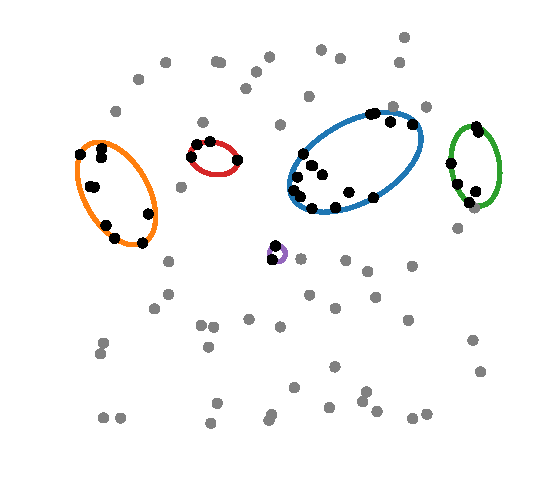
\includegraphics[scale=.8]{tex/figures/AB108}
	\fautor
	\label{fig:AB108}
\end{figure}

As it was said for the results of MCE-$k$, in practice, the bounds for the CLS size and the number of operations taken by the algorithm is very loose.
Notice that, the greatest CLS size was $730$ obtained for the third ellipse in instances CM7-CM9. Notice that $730$ is very distance from its upper-bound $n^3$, which in this case is $10^6$.
Also, looking at the size of the backtracking tree times $n$ as an estimate for the number of computations taken by the algorithm, for example, for instance AB120, this number is $1579 \times 100$, which is very distant from its asymptotic upper-bound of $\bigO(m2^mn^{3m+1})$, which in this case would be $5\times 2^5 \times 100 ^ {16}$.


\section{New instances}

After examining the results obtained by our algorithms for the formerly known instances, constructing new ones, more challenging for our work, can be taken as essential for further analyzing the algorithms proposed by us.
Besides increasing the size of the demand set and the number of ellipses, we also designed instances with non-unitary weights, which is something none of the previous instances had. 
Moreover, to create very distinct instances from the previously introduced ones, we used a different probability distribution, other than the uniform one, to generate the location of points.
We set a time limit of two hours of running time for solving every instance, meaning that if an algorithm did not stop in two hours, we report that it was not able to determine an optimal solution. 
In total, we designed 46 new instances, which will be referred to as TA01, \dots, TA46, and are available at \url{https://sites.icmc.usp.br/andretta/tedeschi-2020/}. The numerical results for every one of them are displayed in \autoref{chapter:tables}.

The first set of instances were construct sampling each demand points from a bivariate normal distribution $\mathcal{N}([0, 0]^T, \mathbb{I})$, with $\mathbb{I} \in \R^{2\times 2}$ being the identity matrix; and setting each point's weight as its squared distance to the origin. This is expected to produce a demand set with most points located near the origin, but with the most valuable points located far away from it.
We generated a set of $n=100$ points, with $m=7$ ellipses, making the $j$-th ellipse have shape parameters randomly taken from a uniform distribution in $[0.5, 1.5]$, and cost $c_j=10\times a_j \times b_j$. From that, we created seven instances taking $k \in \{1, \dots, m\}$. The results for MCE-$k$ can be seen in \autoref{tab:mce-results-ta1} and the results for MCER-$k$ are presented in \autoref{tab:mcer-results-ta1}. 
Because the normal distribution generates most of the points close to each other (see \autoref{fig:TA004} for an example), every ellipse's CLS's size ended up being significantly bigger if compared to previously introduced instances with $100$ points.
This, and the subtle increase in the number of ellipses, made the algorithms for MCER-$k$ and MCE-$k$ time out for some instances. The algorithm for MCER-$k$ did not return an optimal solution within the predefined time limit for the last three instances ($k=5, 6, 7)$, while the algorithm for MCE-$k$ did not finish in time for the last instance ($k=7$). The optimal solution for MCER-$k$ for the instance with $k=4$ is displayed in \autoref{fig:TA004}. 

\begin{figure}[H]
	\centering
	\caption{An optimal solution of MCER-$k$ for the instance TA04.}
	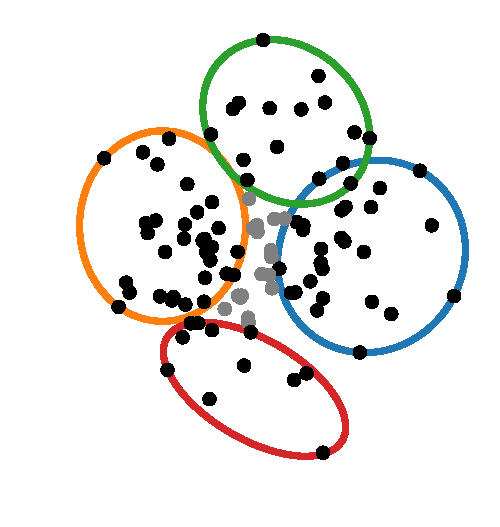
\includegraphics[scale=.8]{tex/figures/TA004}
	\fautor
	\label{fig:TA004}
\end{figure}

For the second set of instances, we used the same process used for the first set to generate the demand points and the ellipses. We kept the number of ellipses at $3$ and created five demand sets with $n\in\{200, 250, 300, 350, 400\}$. In total, we had $15$ instances having $k\in\{1, \dots, m\}$. The results for MCE-$k$ can be seen in \autoref{tab:mce-results-ta2} and the results for MCER-$k$ are presented in \autoref{tab:mcer-results-ta2}. The solution of MCER-$k$ for the instance with $n=400$, and $k=2$ is shown in \autoref{fig:TA021}.

\begin{figure}[H]
	\centering
	\caption{An optimal solution of MCER-$k$ for the instance TA21.}
	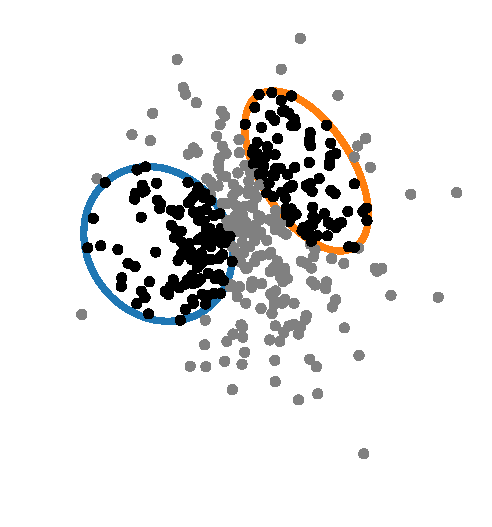
\includegraphics[scale=.8]{tex/figures/TA021}
	\fautor
	\label{fig:TA021}
\end{figure}

The third set of instances were constructed generating the demand set following a uniform distribution in $[0, 10]^2$, with each point having unitary weight; and the ellipses by the same process used for the first two set of instances. We created instances with $m=5$, $n\in \{400, 450, 500\}$, and $k\in\{1, \dots, m\}$, with a total of $15$ instances. The results for MCE-$k$ can be seen in \autoref{tab:mce-results-ta3} and the results for MCER-$k$ are presented in \autoref{tab:mcer-results-ta3}. Optimal solutions were obtained for every one of the instances in this set. It is possible to see that, compared with the first two sets of instances, the CLS sizes are smaller, mostly because of the size of the ellipses and the uniform distribution used to generate the points. The optimal solution returned by MCER-$k$'s algorithm for the instance with $n=500$ and $k=5$ is shown in \autoref{fig:TA037}.

\begin{figure}[!htb]
	\centering
	\caption{An optimal solution of MCER-$k$ for the instance TA37.}
	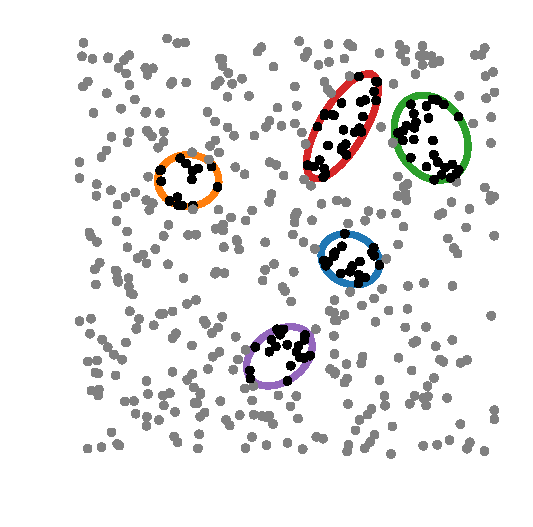
\includegraphics[scale=.8]{tex/figures/TA037}
	\fautor
	\label{fig:TA037}
\end{figure}

The last set of instances were constructed using two bivariate normal distributions with unitary variance $\mathcal{N}(\mu^{(1)}, \mathbb{I})$ and $\mathcal{N}(\mu^{(2)}, \mathbb{I})$, $\mu^{(1)}, \mu^{(2)} \in \R^2$. Half of the points were generated following $\mathcal{N}(\mu^{(1)}, \mathbb{I})$, and the other half $\mathcal{N}(\mu^{(2)}, \mathbb{I})$; the weight of every point was set as its squared distance to the mean of the distribution from which it was generated.
The ellipses were also divided into two halves, taking their shape parameters from uniform distributions in the intervals $[0.5, 1.5]$, and $[3, 4]$; setting the $j$-th ellipse's weight as $c_j=a_j \times b_j$.
The purpose of this last set of instances was to create an example where the chosen ellipses in the solution of an instance of MCER-$k$ is not a subset of the chosen ellipses in an optimal solution of that same instance for MCER-$(k+1)$. We created seven instances with $n=80$, $m=6$ and $k\in\{1, \dots, m\}$, and defined the values of $\mu^{(1)}$ and $\mu^{(2)}$ specifically to create such counter-example. The results are shown in \autoref{tab:mce-results-ta4} for MCE-$k$ and in \autoref{tab:mce-results-ta4} for MCER-$k$.
In \autoref{fig:TA44-45}, we show the solutions for the instances with $k=2$, where two of the bigger-sized ellipses are used, and $k=3$, where one of the bigger-sized ellipses is replaced by two small ones.

\begin{figure}[!htb]
	\caption{Optimal solutions for instances TA44 and TA45.}
	\begin{subfigure}{.5\textwidth}
			\centering
		\caption{TA44}
		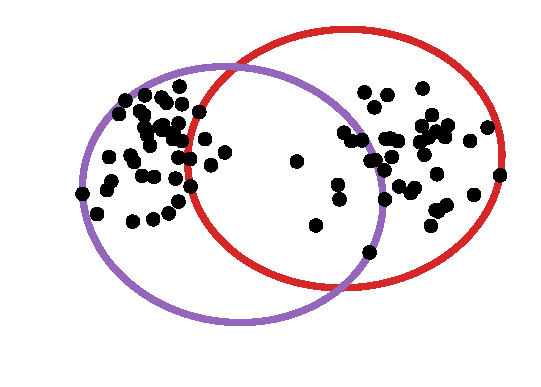
\includegraphics[scale=.8]{tex/figures/TA044}

		%\fautor
		\label{fig:TA043}
	\end{subfigure}
	\begin{subfigure}{.5\textwidth}
			\centering
		\caption{TA45}
		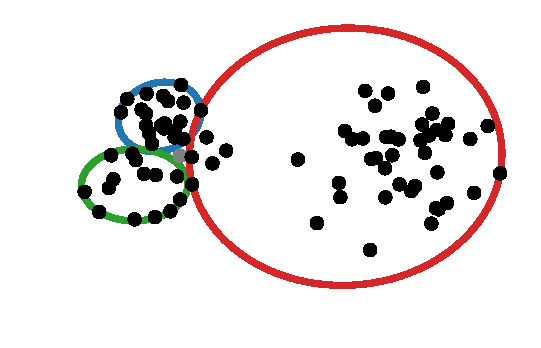
\includegraphics[scale=.8]{tex/figures/TA045}
		%\fautor
		\label{fig:TA044}
	\end{subfigure}
\label{fig:TA44-45}
	\fautor
\end{figure}
